%%===================Método proposto==============%%
\section{Método Proposto}
\subsection{Método Proposto}
\frame{
  \frametitle{Método Proposto}
   
   \begin{block}{Metodologia}
      	\begin{itemize}
      	 \item Esta proposta visa a aplicação da EG para geração de heurísticas
      	 de alto nível para uma plataforma hiper-heurística para o PDP.
      	 \item Baseada no trabalho desenvolvido por Sabar et al. \cite{sabar2015automatic}.
      	 \item No contexto desta proposta:
      	   \begin{itemize}
	      	 \item Heurísticas de alto nível consistem de um \textbf{mecanismo de seleção} e um \textbf{critério de aceitação}. 
	      	 \item Heurísticas de baixo nível são compostas por um conjunto de heurísticas, selecionadas de
	      	 estudos anteriores, um mecanismo de memória e uma função de \textit{fitness}.
      	   \end{itemize}
      	\end{itemize}
   \end{block}
}


\subsection{Método Proposto}
\frame{
	\frametitle{Método Proposto}
	
	\begin{block}{Metodologia}
		
		\begin{figure}[!htb]
			\centering
			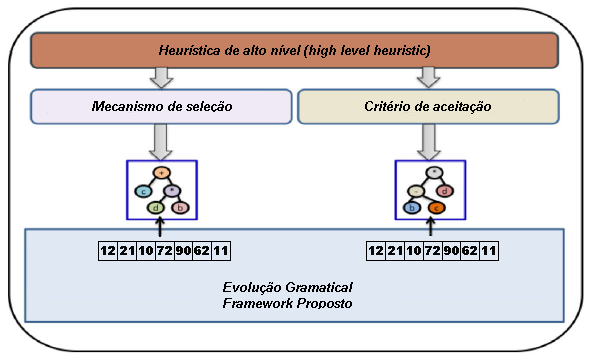
\includegraphics[scale=.8]{figuras/ProposedFramework.png}
			\caption{Método proposto}
			\label{fig:proposedFramework}
		\end{figure}
		
	\end{block}
}

\subsection{Objetivos}
\frame{
	\frametitle{Objetivos}
	
	\begin{block}{Objetivos do trabalho}
			\begin{itemize}
				\item Texto;
				\item Texto;
				\item Texto;
				\item Texto;
				\item Texto.
			\end{itemize}
	\end{block}
	
	\begin{block}{Funções objetivas do trabalho}
		\begin{itemize}
			\item $ maxf_{i}(T)=pc(T) $
			\item $ minf_{ii}(T)=\frac{custo(T)}{nº \; c \; de \; t} $
			\item $ maxf_{iii}(T)=\frac{pref(T)}{nº \; c \; de \; t} $
			\item $ maxf_{iv}(T)=escore(T) $
			\item $ minf_{v}(T)=nCasos(T) $
		\end{itemize}
	\end{block}
}

\frame{
	\frametitle{Funções objetivas do trabalho}
	
	\begin{block}{Funções objetivas do trabalho}
		\begin{itemize}
			\item $ pc(T)=\frac{(nº \; de \; p \; c)}{(nº \; de \; p \; c)}  $
			\item $ c(T)=\displaystyle\sum_{i=0}^{i<n} c(p_{i}) $
			\item $ p(T)=\displaystyle\sum_{i=0}^{i<n} p(p_{i}) $	
			\item $ score(T)=\frac{(nº \; de \; m \; m)}{(nº \; de \; m \; g + nº \; de \; m \; e)} $
			\item $ nCasos(T)=\frac{(nº \; de \; c \; de \; t)}{(total \; de \; p)}  $
		\end{itemize}
	\end{block}
}

\frame{
	\frametitle{\textit{Tabela}}

	\begin{block}{\textit{Tabelas} utilizadas}
	\begin{table}[!htb]
		\renewcommand{\arraystretch}{1.5}
		\fontsize{10pt}{12pt}\selectfont
		\centering
		\scalebox{0.8}{
			\begin{tabular}{c | c | c | c | c }
				\toprule
				\textbf{Matriz} & \textbf{Qtde de P} & \textbf{Qtde de M} & \textbf{Qtde de Pa} & \textbf{Qtde de C}\\ \midrule
				texto1 & 450 & 227 & 183 & 21\\ \midrule
				texto2 & 1152 & 394 & 202 & 22\\ \midrule
				texto3 & 68 & 106 & 75 & 14\\ \midrule
				texto4 & 504 & 357 & 195 & 22\\
				\bottomrule
			\end{tabular}
		}
	\end{table}
	\end{block}
}